% =============================================================================
%  The assumptions of a one-dimensional PBL closure, as a pyramid -- LINKS version
%  GENERATED by scripts/make_pyramid_links.py from pbl_assumptions_pyramid.tex; edit the horizontal
%  file (blocks, frames, \lean entries) and regenerate. Same blocks and contacts; the dependencies
%  the contact rule cannot draw are routed lines: out of the top edge, along a lane above the figure,
%  onto the top edge of the block leaned on; premises are reached round the side and from below.
% =============================================================================
\documentclass[10pt]{article}
\usepackage{iftex}
\ifPDFTeX
  \usepackage[utf8]{inputenc}
  \usepackage[T1]{fontenc}
  \usepackage{lmodern}
\else
  \usepackage{fontspec}
  \setmainfont{lmroman10-regular.otf}[BoldFont=lmroman10-bold.otf,
    ItalicFont=lmroman10-italic.otf, BoldItalicFont=lmroman10-bolditalic.otf]
\fi
\usepackage[british]{babel}
\usepackage[paperwidth=32cm,paperheight=21cm,margin=8mm]{geometry}
\usepackage{amsmath,amssymb}
\usepackage{xcolor}
\usepackage{tikz}
\usetikzlibrary{arrows.meta}
\usepackage{microtype}
\pagestyle{empty}
\setlength{\parindent}{0pt}
\setlength{\parskip}{0.5ex}
% rigid math relation spacing: the centred block texts would otherwise stretch around = and <<
\thickmuskip=5mu \medmuskip=4mu \thinmuskip=3mu

% ---- notation ---------------------------------------------------------------
\newcommand{\avg}[1]{\langle #1 \rangle}
\newcommand{\pd}[2]{\partial #1/\partial #2}
\newcommand{\qsq}{q^{2}}
\newcommand{\Rfc}{R_{fc}}
\newcommand{\dx}{\Delta x}
% ---- rows the PhD concept turns on (same data as the note's macros.tex) ------
\definecolor{cKey}{HTML}{7B2D8E}
\definecolor{cGXIX}{HTML}{990011}   % Goger 2019 port (the note's colour)
\definecolor{cFULL}{HTML}{7B2D8E}   % Kosovic-Juliano 3D closure (the note's colour)
% \hl{x0}{x1}{y0}{y1}{colour}{inset}: a frame inside a block, marking a scheme's decisive block
\newcommand{\hl}[6]{\draw[#5, line width=1.1pt] (#1+#6,#3+#6) rectangle (#2-#6,#4-#6);}
\newcommand{\setkey}[2]{\expandafter\def\csname key@#1\endcsname{#2}}
\makeatletter
\setkey{A1}{1}\setkey{B1}{1}\setkey{B2}{1}\setkey{B3}{1}\setkey{C3}{1}\setkey{C4}{1}\setkey{C6}{1}\setkey{C7}{1}
\setkey{B5}{2}\setkey{B6}{2}\setkey{C2}{2}\setkey{C5}{2}\setkey{C9}{2}
\newcommand{\keymark}[1]{\ifcsname key@#1\endcsname
  \if1\csname key@#1\endcsname\textcolor{cKey}{$\blacktriangleright$}\else\textcolor{cKey}{$\triangleright$}\fi\fi}
\makeatother
\newcommand{\pid}[1]{\keymark{#1}\textbf{#1}}
% \pb{x0}{x1}{y0}{y1}{style}{text}: a block from (x0,y0) to (x1,y1), text centred
\newcommand{\pbf}[7]{\pgfmathsetmacro{\pbw}{#2-#1-#7}%
  \draw[#5] (#1,#3) rectangle (#2,#4);
  \node[align=center, font=\tiny, inner sep=0pt, text width=\pbw cm] at ({(#1+#2)/2},{(#3+#4)/2}) {#6};}
\newcommand{\pb}[6]{\pgfmathsetmacro{\pbw}{#2-#1-0.20}%
  \draw[#5] (#1,#3) rectangle (#2,#4);
  \node[align=center, font=\tiny, inner sep=0pt, text width=\pbw cm] at ({(#1+#2)/2},{(#3+#4)/2}) {#6};}


% ---- the hectometre-scale column (used by the VERTICAL version only; read by scripts/make_pyramid_vertical.py)
% \hecto{<concept title>}{<what becomes of the concept at Delta = 500 m over the Inn Valley>}; no-op here.
% Sources: the mountain and grey-zone columns of the note's Table I.1 and the project's own runs.
\newcommand{\hecto}[2]{}
\hecto{Locality}{By day eddies span $z_i$ and the flux stops answering the local gradient; on slopes it arrives from the interface. Holds at night.}
\hecto{Reynolds averaging}{The cell mean is a filter of width $\Delta$ inside the spectrum: Leonard and cross terms appear; the closed term is a subfilter stress.}
\hecto{Ergodicity in space}{At night a 500~m cell holds about five integral scales per direction and $\Delta z$ none: the cell statistic is an order-one realisation. By day it holds less than one eddy. On a slope it mixes two flows, slope layer and valley core, and estimates neither.}
\hecto{Boundary-layer (column) approximation}{Not small: the cross-valley shear of the up-valley jet reaches 20--30\,\% of the vertical shear; slope flows carry $W$ gradients of the order of the wind shear; horizontal flux divergences are of the order of the vertical one, and the Riviera budgets closed only with transport and advection. Seven of nine production terms and the three-dimensional divergences are missing, not negligible.}
\hecto{Constant-flux layer}{The katabatic jet nose at 2--10~m sits inside the layer; the momentum flux is height-constant in 8--28\,\% of daytime periods.}
\hecto{Local equilibrium}{Resolved strain by day rotates faster than $l/q$; transitions and intermittency at night are not slow against it.}
\hecto{Monin--Obukhov similarity}{A slope has two axes, gravity and the surface normal: two Obukhov lengths, a slope-normal heat flux with a horizontal part. The scaling holds only for some anisotropy classes, and over a hill only in the inner layer. Over the forested slopes the first model level sits inside the roughness sublayer. At Innsbruck the surface is stable 4.7\,\% of the time while the valley air above is often stably stratified.}
\hecto{Mixing length}{$z_i$ ill-posed under elevated inversions, wall distance ambiguous on a slope; the valley width sets the horizontal eddy: two lengths.}
\hecto{Universal constants}{Fitted to flat neutral and convective layers; the anisotropy classes of complex terrain differ, and the comparison already runs three constant sets. Filter constants are not ensemble constants: $C_\varepsilon$ depends on $l/\Delta$.}
\hecto{Energy cascade}{$\varepsilon$ is filter-independent while $q^3$ is not: the dissipation length must shrink with the grid; by day the filter cuts into the isotropic range.}
\hecto{Return to isotropy}{Stable valley turbulence is two-component, pancake-like; the return rate of a pancake need not be that of a convective eddy. Pressure work by slope flows and gravity waves redistributes energy laterally, the least known term of the budget.}
\hecto{Eddy viscosity}{The grid filter, aspect ratio 25, imprints its anisotropy on the subgrid eddies; the stress axes turn where slope meets valley wind.}
\hecto{Buoyancy production}{The slope-normal surface heat flux has a horizontal component with no home in the budget; in stable air buoyancy damps $\avg{w^2}$ selectively, the pancake anisotropy; by day resolved thermals carry the horizontal heat flux and its subgrid part stays unrepresented.}


% ---- dependencies the contact rule cannot draw (used by the LINKS version only; scripts/make_pyramid_links.py)
% \lean{<block title>}{<block title it leans on>}; from the audit of 2026-09-16. No-op here.
\newcommand{\lean}[2]{}
\lean{Locality}{Mixing}
\lean{Ergodicity in space}{Scale separation}
\lean{Boundary-layer (column) approximation}{Boussinesq}
\lean{Monin--Obukhov similarity}{Horizontal homogeneity}
\lean{Monin--Obukhov similarity}{Axisymmetry}
\lean{Mixing length}{Horizontal homogeneity}
\lean{Energy cascade}{Stationarity}
\lean{Local equilibrium}{Locality}
\lean{Eddy viscosity}{Locality}
\lean{Universal constants}{Reynolds averaging}
\lean{Vertical divergence only}{Scale separation}
\lean{Wall value and surface fluxes}{Monin--Obukhov similarity}
\lean{Wall value and surface fluxes}{Universal constants}
\lean{Level-2.5 truncation}{Return to isotropy}
\lean{Level-2.5 truncation}{Universal constants}
\lean{Level-2.5 truncation}{Boundary-layer (column) approximation}
\lean{Master length scale}{Universal constants}
\lean{Master length scale}{Axisymmetry}
\lean{Pressure terms}{Locality}
\lean{Pressure terms}{Universal constants}
\lean{K-form fluxes}{Locality}
\lean{K-form fluxes}{Mixing length}
\lean{K-form fluxes}{Local equilibrium}
\lean{Dissipation}{Master length scale}
\lean{Resolved gradient}{Boundary-layer (column) approximation}


\definecolor{cLinkF}{HTML}{1F5FA8}   % a formal statement leaning on something undrawn
\definecolor{cLinkC}{HTML}{2E7D32}   % a concept leaning on something undrawn
\tikzset{link/.style={line width=0.5pt, rounded corners=3pt, -{Stealth[length=3.5pt, width=2.8pt]}, opacity=0.85}}

\begin{document}
{\Large\bfseries The assumptions of a one-dimensional PBL closure, as a pyramid: what rests on what, with every dependency}\\[0.3ex]
{\small Companion page with the dependencies the contact rule cannot draw added as lines. 2026-09-16.}

\vspace{0.6ex}
{\footnotesize Blocks and contacts as on the companion page: a block touches at its bottom exactly its primary
parents. The lines are the remaining dependencies from the audit of the same day. A line leaves a block through
its top edge, at a spot no block covers where one exists, runs along a lane above the figure and arrives on the top
edge of the block it leans on; a premise is reached round the side and from below. \textcolor{cLinkF}{\textbf{Blue}}:
a formal statement leaning on a concept or a premise; \textcolor{cLinkC}{\textbf{green}}: a concept leaning on a
premise or on another concept; dashed: within one tier. Not drawable because they are not blocks: small-scale
isotropy and the cascade presuppose a high Reynolds number, the buoyancy term presupposes unsaturated air. Drawn:
\textit{Locality} on Mixing; \textit{Ergodicity in space} on Scale separation; \textit{Boundary-layer (column) approximation} on Boussinesq; \textit{Monin--Obukhov similarity} on Horizontal homogeneity, Axisymmetry; \textit{Mixing length} on Horizontal homogeneity; \textit{Energy cascade} on Stationarity; \textit{Local equilibrium} on Locality; \textit{Eddy viscosity} on Locality; \textit{Universal constants} on Reynolds averaging; \textit{Vertical divergence only} on Scale separation; \textit{Wall value and surface fluxes} on Monin--Obukhov similarity, Universal constants; \textit{Level-2.5 truncation} on Return to isotropy, Universal constants, Boundary-layer (column) approximation; \textit{Master length scale} on Universal constants, Axisymmetry; \textit{Pressure terms} on Locality, Universal constants; \textit{K-form fluxes} on Locality, Mixing length, Local equilibrium; \textit{Dissipation} on Master length scale; \textit{Resolved gradient} on Boundary-layer (column) approximation.\par}

\vspace{0.8ex}
\begin{center}
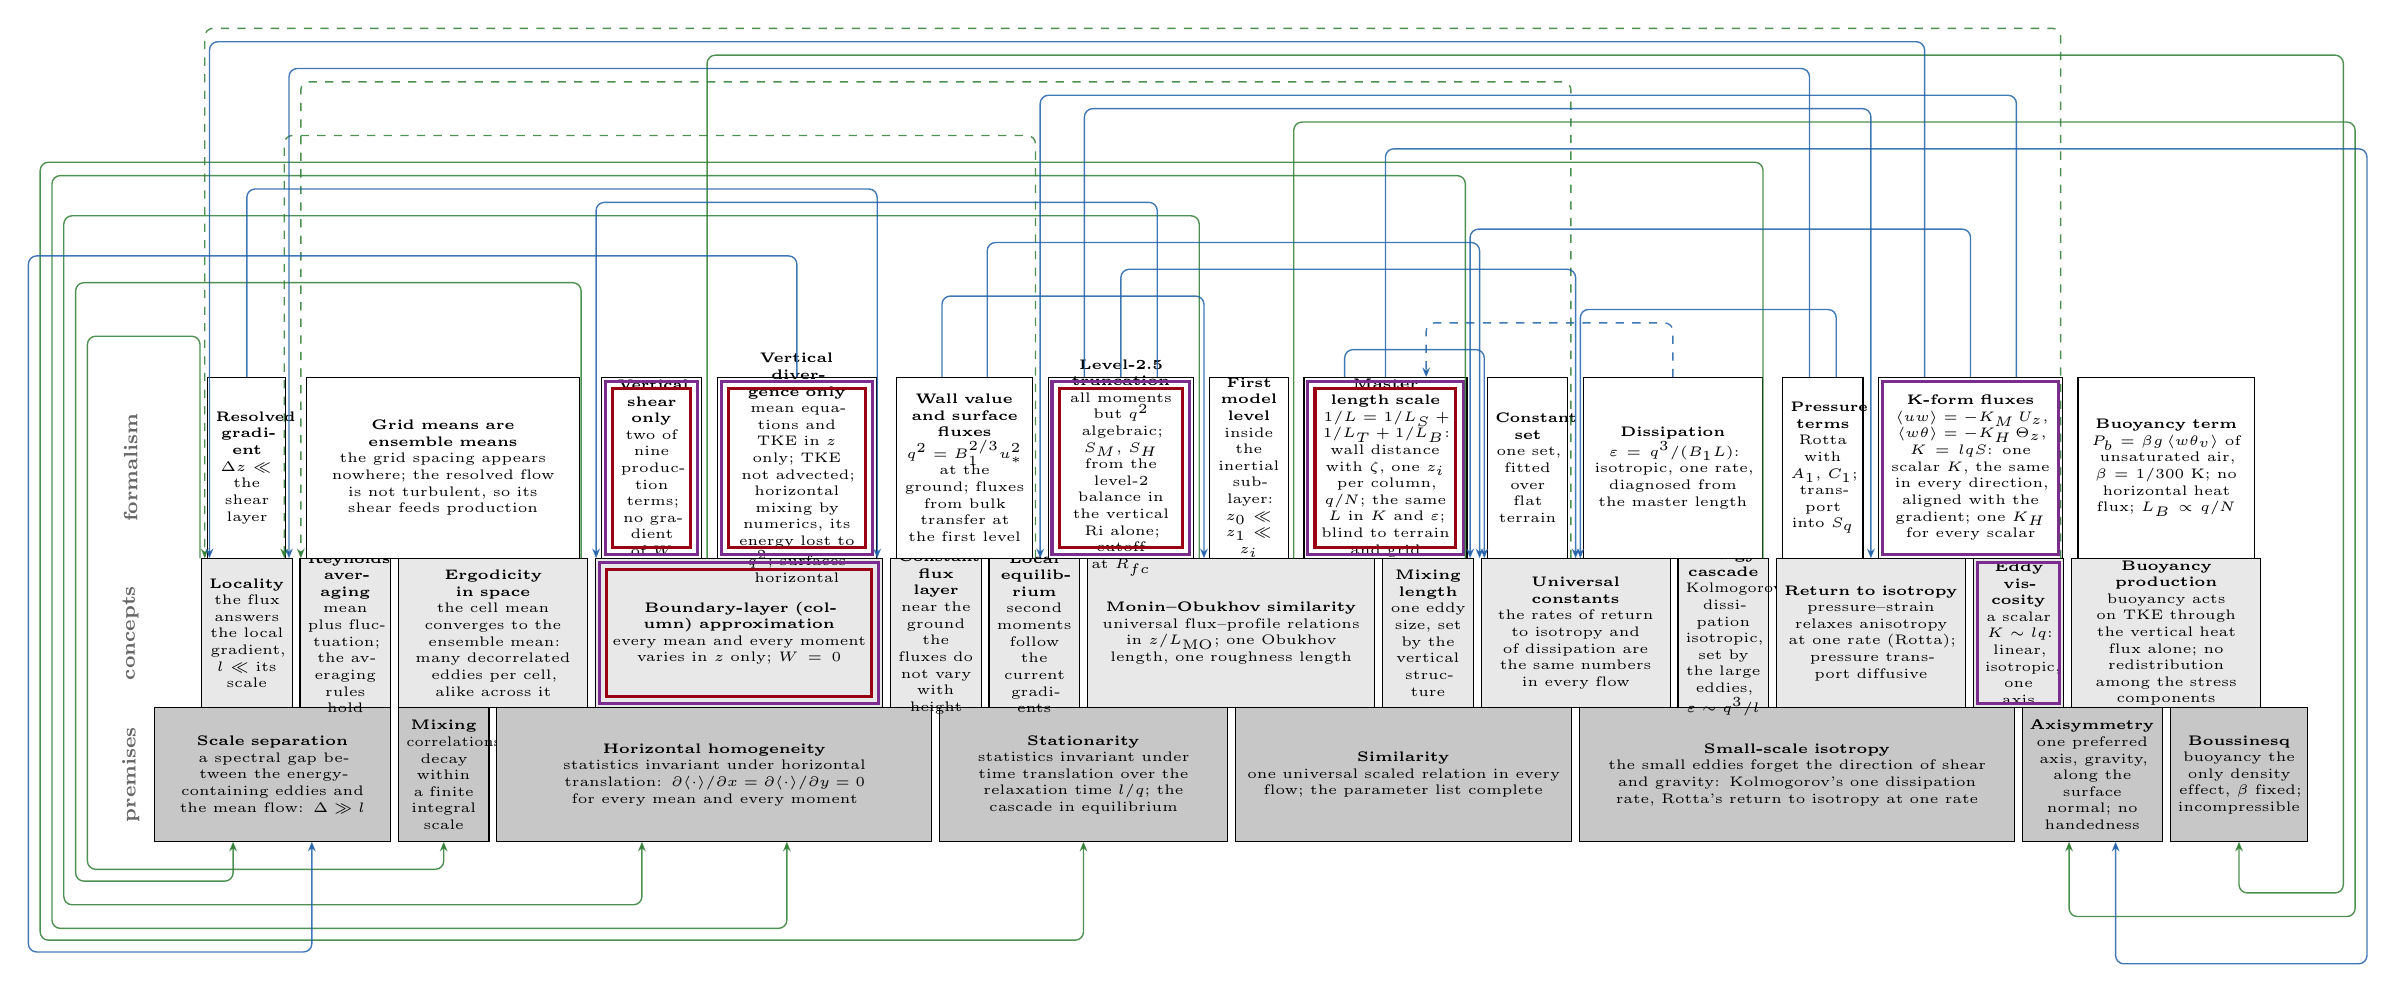
\begin{tikzpicture}[x=1cm, y=1cm,
  ground/.style={draw, line width=0.4pt, fill=black!22},
  hyp/.style={draw, line width=0.4pt, fill=black!9},
  row/.style={draw, line width=0.4pt, fill=white},
  tier/.style={font=\scriptsize\bfseries, rotate=90, anchor=center, text=black!60}]
% ---- tier labels -----------------------------------------------------------------------------------
\node[tier] at (-0.3, 0.85) {premises};
\node[tier] at (-0.3, 2.65) {concepts};
\node[tier] at (-0.3, 4.75) {formalism};
% ---- tier 0: physical hypotheses (y 0 -- 1.7); each boundary sits under the concept that spans it --
% order forced by the adjacency chain SEP-MIX-HOM-STA-SIM-ISOb-AXI-BOU (unit 1.15, gap 0.10, offset 0.6)
\pb{0}{3.00}{0}{1.7}{ground}{\textbf{Scale separation}\\ a spectral gap between the energy-containing eddies and the mean flow: \mbox{$\Delta \gg l$}}
\pb{3.10}{4.25}{0}{1.7}{ground}{\textbf{Mixing}\\ correlations decay within a finite integral scale}
\pb{4.35}{9.875}{0}{1.7}{ground}{\textbf{Horizontal homogeneity}\\ statistics invariant under horizontal translation: \mbox{$\pd{\avg{\cdot}}{x} = \pd{\avg{\cdot}}{y} = 0$} for every mean and every moment}
\pb{9.975}{13.625}{0}{1.7}{ground}{\textbf{Stationarity}\\ statistics invariant under time translation over the relaxation time $l/q$; the cascade in equilibrium}
\pb{13.725}{18.00}{0}{1.7}{ground}{\textbf{Similarity}\\ one universal scaled relation in every flow; the parameter list complete}
\pb{18.10}{23.625}{0}{1.7}{ground}{\textbf{Small-scale isotropy}\\ the small eddies forget the direction of shear and gravity: Kolmogorov's one dissipation rate, Rotta's return to isotropy at one rate}
\pb{23.725}{25.50}{0}{1.7}{ground}{\textbf{Axisymmetry}\\ one preferred axis, gravity, along the surface normal; no handedness}
\pb{25.60}{27.35}{0}{1.7}{ground}{\textbf{Boussinesq}\\ buoyancy the only density effect, $\beta$ fixed; incompressible}
% ---- tier 1: concepts (y 1.7 -- 3.6); 7 singles of 1.15, 4 doubles of 2.40, 2 triples of 3.65 ------
\pb{0.60}{1.75}{1.7}{3.6}{hyp}{\textbf{Locality}\\ the flux answers the local gradient, $l \ll$ its scale}
\pb{1.85}{3.00}{1.7}{3.6}{hyp}{\textbf{Reynolds averaging}\\ mean plus fluctuation; the averaging rules hold}
\pb{3.10}{5.50}{1.7}{3.6}{hyp}{\textbf{Ergodicity in space}\\ the cell mean converges to the ensemble mean: many decorrelated eddies per cell, alike across it}
\pbf{5.60}{9.25}{1.7}{3.6}{hyp}{\textbf{Boundary-layer (column) approximation}\\ every mean and every moment varies in $z$ only; $W = 0$}{0.44}
\pb{9.35}{10.50}{1.7}{3.6}{hyp}{\textbf{Constant-flux layer}\\ near the ground the fluxes do not vary with height}
\pb{10.60}{11.75}{1.7}{3.6}{hyp}{\textbf{Local equilibrium}\\ second moments follow the current gradients}
\pb{11.85}{15.50}{1.7}{3.6}{hyp}{\textbf{Monin--Obukhov similarity}\\ universal flux--profile relations in $z/L_{\mathrm{MO}}$; one Obukhov length, one roughness length}
\pb{15.60}{16.75}{1.7}{3.6}{hyp}{\textbf{Mixing length}\\ one eddy size, set by the vertical structure}
\pb{16.85}{19.25}{1.7}{3.6}{hyp}{\textbf{Universal constants}\\ the rates of return to isotropy and of dissipation are the same numbers in every flow}
\pb{19.35}{20.50}{1.7}{3.6}{hyp}{\textbf{Energy cascade}\\ Kolmogorov: dissipation isotropic, set by the large eddies, $\varepsilon \sim q^3/l$}
\pb{20.60}{23.00}{1.7}{3.6}{hyp}{\textbf{Return to isotropy}\\ pressure--strain relaxes anisotropy at one rate (Rotta); pressure transport diffusive}
\pbf{23.10}{24.25}{1.7}{3.6}{hyp}{\textbf{Eddy viscosity}\\ a scalar $K \sim l q$: linear, isotropic, one axis}{0.30}
\pb{24.35}{26.75}{1.7}{3.6}{hyp}{\textbf{Buoyancy production}\\ buoyancy acts on TKE through the vertical heat flux alone; no redistribution among the stress components}
% ---- tier 2: the formalism (y 3.6 -- 5.9) --------------------------------------------------------------
\pb{0.68}{1.67}{3.6}{5.9}{row}{\textbf{Resolved gradient}\\ $\Delta z \ll$ the shear layer}
\pb{1.93}{5.40}{3.6}{5.9}{row}{\textbf{Grid means are ensemble means}\\ the grid spacing appears nowhere; the resolved flow is not turbulent, so its shear feeds production}
\pbf{5.68}{6.95}{3.6}{5.9}{row}{\textbf{Vertical shear only}\\ two of nine production terms; no gradient of $W$}{0.44}
\pbf{7.15}{9.17}{3.6}{5.9}{row}{\textbf{Vertical divergence only}\\ mean equations and TKE in $z$ only; TKE not advected; horizontal mixing by numerics, its energy lost to $\qsq$; surfaces horizontal}{0.44}
\pb{9.43}{11.15}{3.6}{5.9}{row}{\textbf{Wall value and surface fluxes}\\ $\qsq = B_1^{2/3} u_*^2$ at the ground; fluxes from bulk transfer at the first level}
\pbf{11.35}{13.20}{3.6}{5.9}{row}{\textbf{Level-2.5 truncation}\\ all moments but $\qsq$ algebraic; $S_M$, $S_H$ from the level-2 balance in the vertical Ri alone; cutoff at $\Rfc$}{0.44}
\pb{13.40}{14.40}{3.6}{5.9}{row}{\textbf{First model level}\\ inside the inertial sublayer: $z_0 \ll z_1 \ll z_i$}
\pbf{14.60}{16.67}{3.6}{5.9}{row}{\textbf{Master length scale}\\ $1/L = 1/L_S + 1/L_T + 1/L_B$: wall distance with $\zeta$, one $z_i$ per column, $q/N$; the same $L$ in $K$ and $\varepsilon$; blind to terrain and grid}{0.44}
\pb{16.93}{17.95}{3.6}{5.9}{row}{\textbf{Constant set}\\ one set, fitted over flat terrain}
\pb{18.15}{20.42}{3.6}{5.9}{row}{\textbf{Dissipation}\\ $\varepsilon = q^3/(B_1 L)$: isotropic, one rate, diagnosed from the master length}
\pb{20.68}{21.70}{3.6}{5.9}{row}{\textbf{Pressure terms}\\ Rotta with $A_1$, $C_1$; transport into $S_q$}
\pbf{21.90}{24.23}{3.6}{5.9}{row}{\textbf{K-form fluxes}\\ \mbox{$\avg{uw} = -K_M\,U_z$}, \mbox{$\avg{w\theta} = -K_H\,\Theta_z$}, $K = l q S$: one scalar $K$, the same in every direction, aligned with the gradient; one $K_H$ for every scalar}{0.30}
\pb{24.43}{26.67}{3.6}{5.9}{row}{\textbf{Buoyancy term}\\ $P_b = \beta g\,\avg{w\theta_v}$ of unsaturated air, $\beta = 1/300$~K; no horizontal heat flux; $L_B \propto q/N$}
% ---- decisive blocks of the two schemes run in the comparison (the framed cells of the note's Table I.0) ---
% purple = Kosovic-Juliano 3D closure (outer), red = Goger 2019 port (inner); both = nested
\hl{5.60}{9.25}{1.7}{3.6}{cFULL}{0.05}\hl{5.60}{9.25}{1.7}{3.6}{cGXIX}{0.14}     % column approximation
\hl{5.68}{6.95}{3.6}{5.9}{cFULL}{0.05}\hl{5.68}{6.95}{3.6}{5.9}{cGXIX}{0.14}     % vertical shear only
\hl{7.15}{9.17}{3.6}{5.9}{cFULL}{0.05}\hl{7.15}{9.17}{3.6}{5.9}{cGXIX}{0.14}     % vertical divergence only
\hl{11.35}{13.20}{3.6}{5.9}{cFULL}{0.05}\hl{11.35}{13.20}{3.6}{5.9}{cGXIX}{0.14} % level-2.5 truncation (cutoff)
\hl{14.60}{16.67}{3.6}{5.9}{cFULL}{0.05}\hl{14.60}{16.67}{3.6}{5.9}{cGXIX}{0.14} % master length scale
\hl{23.10}{24.25}{1.7}{3.6}{cFULL}{0.05}                                          % eddy viscosity (3D only)
\hl{21.90}{24.23}{3.6}{5.9}{cFULL}{0.05}                                          % K-form fluxes (3D only)
\draw[link, cLinkC] (0.580,3.60) -- (0.580,6.42) -- (-0.85,6.42) -- (-0.85,-0.35) -- (3.675,-0.35) -- (3.675,0.00);  % Locality -> Mixing
\draw[link, cLinkC] (5.420,3.60) -- (5.420,7.10) -- (-1.00,7.10) -- (-1.00,-0.50) -- (1.000,-0.50) -- (1.000,0.00);  % Ergodicity in space -> Scale separation
\draw[link, cLinkC] (7.020,3.60) -- (7.020,9.99) -- (27.80,9.99) -- (27.80,-0.65) -- (26.475,-0.65) -- (26.475,0.00);  % Boundary-layer (column) approximation -> Boussinesq
\draw[link, cLinkC] (13.270,3.60) -- (13.270,7.95) -- (-1.15,7.95) -- (-1.15,-0.80) -- (6.192,-0.80) -- (6.192,0.00);  % Monin--Obukhov similarity -> Horizontal homogeneity
\draw[link, cLinkC] (14.470,3.60) -- (14.470,9.14) -- (27.95,9.14) -- (27.95,-0.95) -- (24.317,-0.95) -- (24.317,0.00);  % Monin--Obukhov similarity -> Axisymmetry
\draw[link, cLinkC] (16.650,3.60) -- (16.650,8.46) -- (-1.30,8.46) -- (-1.30,-1.10) -- (8.033,-1.10) -- (8.033,0.00);  % Mixing length -> Horizontal homogeneity
\draw[link, cLinkC] (20.430,3.60) -- (20.430,8.63) -- (-1.45,8.63) -- (-1.45,-1.25) -- (11.800,-1.25) -- (11.800,0.00);  % Energy cascade -> Stationarity
\draw[link, cLinkC, dashed] (11.190,3.60) -- (11.190,8.97) -- (1.650,8.97) -- (1.650,3.60);  % Local equilibrium -> Locality
\draw[link, cLinkC, dashed] (24.210,3.60) -- (24.210,10.33) -- (0.640,10.33) -- (0.640,3.60);  % Eddy viscosity -> Locality
\draw[link, cLinkC, dashed] (17.990,3.60) -- (17.990,9.65) -- (1.860,9.65) -- (1.860,3.60);  % Universal constants -> Reynolds averaging
\draw[link, cLinkF] (8.160,5.90) -- (8.160,7.44) -- (-1.60,7.44) -- (-1.60,-1.40) -- (2.000,-1.40) -- (2.000,0.00);  % Vertical divergence only -> Scale separation
\draw[link, cLinkF] (10.003,5.90) -- (10.003,6.93) -- (13.330,6.93) -- (13.330,3.60);  % Wall value and surface fluxes -> Monin--Obukhov similarity
\draw[link, cLinkF] (10.577,5.90) -- (10.577,7.61) -- (16.830,7.61) -- (16.830,3.60);  % Wall value and surface fluxes -> Universal constants
\draw[link, cLinkF] (11.812,5.90) -- (11.812,9.31) -- (21.800,9.31) -- (21.800,3.60);  % Level-2.5 truncation -> Return to isotropy
\draw[link, cLinkF] (12.275,5.90) -- (12.275,7.27) -- (18.050,7.27) -- (18.050,3.60);  % Level-2.5 truncation -> Universal constants
\draw[link, cLinkF] (12.737,5.90) -- (12.737,8.12) -- (5.610,8.12) -- (5.610,3.60);  % Level-2.5 truncation -> Boundary-layer (column) approximation
\draw[link, cLinkF] (15.117,5.90) -- (15.117,6.25) -- (16.890,6.25) -- (16.890,3.60);  % Master length scale -> Universal constants
\draw[link, cLinkF] (15.635,5.90) -- (15.635,8.80) -- (28.10,8.80) -- (28.10,-1.55) -- (24.908,-1.55) -- (24.908,0.00);  % Master length scale -> Axisymmetry
\draw[link, cLinkF] (21.020,5.90) -- (21.020,9.82) -- (1.710,9.82) -- (1.710,3.60);  % Pressure terms -> Locality
\draw[link, cLinkF] (21.360,5.90) -- (21.360,6.76) -- (18.110,6.76) -- (18.110,3.60);  % Pressure terms -> Universal constants
\draw[link, cLinkF] (22.482,5.90) -- (22.482,10.16) -- (0.700,10.16) -- (0.700,3.60);  % K-form fluxes -> Locality
\draw[link, cLinkF] (23.065,5.90) -- (23.065,7.78) -- (16.710,7.78) -- (16.710,3.60);  % K-form fluxes -> Mixing length
\draw[link, cLinkF] (23.648,5.90) -- (23.648,9.48) -- (11.250,9.48) -- (11.250,3.60);  % K-form fluxes -> Local equilibrium
\draw[link, cLinkF, dashed] (19.285,5.90) -- (19.285,6.59) -- (16.152,6.59) -- (16.152,5.90);  % Dissipation -> Master length scale
\draw[link, cLinkF] (1.175,5.90) -- (1.175,8.29) -- (9.180,8.29) -- (9.180,3.60);  % Resolved gradient -> Boundary-layer (column) approximation
\end{tikzpicture}
\end{center}


\vspace{0.6ex}
{\footnotesize\textbf{Frames.} The blocks each scheme's design turns on, the framed cells of the note's Table~I.0,
in the note's scheme colours. \textcolor{cGXIX}{\textbf{Red}}, the Goger 2019 port: it adds a horizontal
shear-production source to the TKE budget (vertical shear only), pays it with the energy the numerical
horizontal operator would otherwise lose and advects TKE (vertical divergence only), gives the source its own
horizontal length from the flow, $l_h^2 = U^2 T_{L,u} T_{L,v}$ (master length scale), and adds a source that knows no
Richardson number to a scheme that keeps the cutoff (level-2.5 truncation); at the concept level it breaks the
column approximation for production alone and keeps every other block. \textcolor{cFULL}{\textbf{Purple}}, the
Kosovi\'c--Juliano three-dimensional closure: it drops the column approximation entirely --- nine production
terms, three-dimensional divergences and TKE transport, metric-corrected gradients, all subgrid mixing from the
closure --- and replaces the eddy viscosity and the K-form by the solved algebraic stress tensor, so no $K$, no
alignment, no stability functions and no cutoff; the equilibrium follows from the full strain. It keeps the master
length scale, one scalar $l$ for the whole tensor: the last one-dimensional block in a three-dimensional scheme, and
the frontier. Nested frames: both schemes; every block the Goger port touches, the three-dimensional closure touches
too, and it alone reaches the eddy viscosity and the K-form.\par}

\vspace{0.4ex}
{\footnotesize\textbf{Reading.} The ground holds the premises, hypotheses about the fluid and the flow; nothing in it names a model. The middle tier is where
the model's vocabulary is born: scale separation gives Reynolds averaging and locality; mixing with homogeneity gives ergodicity in space; homogeneity gives the
column approximation and, with stationarity, the constant-flux layer; stationarity gives local equilibrium and,
with similarity, Monin--Obukhov similarity; similarity gives the mixing length and, with small-scale isotropy,
universal constants; small-scale isotropy gives the cascade, the return to isotropy and, with one axis, a scalar
eddy viscosity; one axis and a Boussinesq fluid give buoyancy production through the vertical heat flux. The top
tier is the closure as written, and every one of its statements applies one or two concepts: the truncation
applies local equilibrium and takes its stability functions from the surface-layer relations they were fitted
to; the master length takes its wall branch from Monin--Obukhov similarity and its shape from the mixing length;
the dissipation takes its form from the cascade and its constant from universality; the K-form takes its scalar
from the eddy viscosity and its coefficients from the return to isotropy. Terrain breaks the ground on the left
and in the middle --- homogeneity, the column, the constant-flux layer, one axis --- and the grey zone breaks it
on the far left; the right third, isotropy and its constants, is the part no scheme in the comparison touches.\par}

\vspace{0.5ex}
{\footnotesize\textbf{Correspondence to the note's rows.} Grid means are ensemble means: A1, A2. Vertical shear only: B1, B2. Vertical divergence only: B3, B4, B5, B7. Constant-flux layer with Monin--Obukhov similarity:
B6, split because one block cannot touch three foundations. Wall value and surface fluxes: the lower boundary of
the TKE equation (D6). First model level: D3. Resolved gradient: D4. K-form fluxes: C1, C2, C3 and the mixing of
all scalars alike. Master length scale: C4 with the one-length statement of C5. Dissipation: C5. Level-2.5
truncation: C6, C7. Buoyancy term: C8 with the dry buoyancy flux (D5). Constant set: C9. Pressure terms: C10.
Which scheme drops which statement is Table~I.0 of the note.\par}

\end{document}
